\PassOptionsToPackage{unicode=true}{hyperref} % options for packages loaded elsewhere
\PassOptionsToPackage{hyphens}{url}
%
\documentclass[ignorenonframetext,]{beamer}
\usepackage{pgfpages}
\setbeamertemplate{caption}[numbered]
\setbeamertemplate{caption label separator}{: }
\setbeamercolor{caption name}{fg=normal text.fg}
\beamertemplatenavigationsymbolsempty
% Prevent slide breaks in the middle of a paragraph:
\widowpenalties 1 10000
\raggedbottom
\setbeamertemplate{part page}{
\centering
\begin{beamercolorbox}[sep=16pt,center]{part title}
  \usebeamerfont{part title}\insertpart\par
\end{beamercolorbox}
}
\setbeamertemplate{section page}{
\centering
\begin{beamercolorbox}[sep=12pt,center]{part title}
  \usebeamerfont{section title}\insertsection\par
\end{beamercolorbox}
}
\setbeamertemplate{subsection page}{
\centering
\begin{beamercolorbox}[sep=8pt,center]{part title}
  \usebeamerfont{subsection title}\insertsubsection\par
\end{beamercolorbox}
}
\AtBeginPart{
  \frame{\partpage}
}
\AtBeginSection{
  \ifbibliography
  \else
    \frame{\sectionpage}
  \fi
}
\AtBeginSubsection{
  \frame{\subsectionpage}
}
\usepackage{lmodern}
\usepackage{amssymb,amsmath}
\usepackage{ifxetex,ifluatex}
\usepackage{fixltx2e} % provides \textsubscript
\ifnum 0\ifxetex 1\fi\ifluatex 1\fi=0 % if pdftex
  \usepackage[T1]{fontenc}
  \usepackage[utf8]{inputenc}
  \usepackage{textcomp} % provides euro and other symbols
\else % if luatex or xelatex
  \usepackage{unicode-math}
  \defaultfontfeatures{Ligatures=TeX,Scale=MatchLowercase}
\fi
\usetheme[]{Montpellier}
\usecolortheme{dolphin}
\usefonttheme{structurebold}
% use upquote if available, for straight quotes in verbatim environments
\IfFileExists{upquote.sty}{\usepackage{upquote}}{}
% use microtype if available
\IfFileExists{microtype.sty}{%
\usepackage[]{microtype}
\UseMicrotypeSet[protrusion]{basicmath} % disable protrusion for tt fonts
}{}
\IfFileExists{parskip.sty}{%
\usepackage{parskip}
}{% else
\setlength{\parindent}{0pt}
\setlength{\parskip}{6pt plus 2pt minus 1pt}
}
\usepackage{hyperref}
\hypersetup{
            pdftitle={Mean comparison tests},
            pdfauthor={Jacques van Helden},
            pdfborder={0 0 0},
            breaklinks=true}
\urlstyle{same}  % don't use monospace font for urls
\newif\ifbibliography
\usepackage{longtable,booktabs}
\usepackage{caption}
% These lines are needed to make table captions work with longtable:
\makeatletter
\def\fnum@table{\tablename~\thetable}
\makeatother
\setlength{\emergencystretch}{3em}  % prevent overfull lines
\providecommand{\tightlist}{%
  \setlength{\itemsep}{0pt}\setlength{\parskip}{0pt}}
\setcounter{secnumdepth}{0}

% set default figure placement to htbp
\makeatletter
\def\fps@figure{htbp}
\makeatother


\title{Mean comparison tests}
\providecommand{\subtitle}[1]{}
\subtitle{Probabilities and statistics for modelling (CMB STAT1)}
\author{Jacques van Helden}
\date{2020-03-06}

\begin{document}
\frame{\titlepage}

\begin{frame}
\tableofcontents[hideallsubsections]
\end{frame}
\begin{frame}{Contents}
\protect\hypertarget{contents}{}

We provide here a brief summary (suppsedly reminder) of one ot the most
popular applications of statistics: the \textbf{mean comparison test}.

This test is used in a wide number of contexts. We will apply it here to
two data types.

\begin{enumerate}
\item
  \textbf{Artificial data} generated by drawing samples from two
  normally distributed populations, having either equal (\(H_0\)) or
  different (\(H_1\)) means depending on the cases. The interest of this
  experiment is that we conrol all the parameters (we know whether there
  is or not a difference betwen population means).
\item
  \textbf{Trabscriptome data obtained from microarrays}. We will test if
  a given gene presents a significant difference between two sets of
  biological samples (e.g.~patients suffering from different cancer
  types).

  \textbf{Note:} microarray technologies have been widely replaced by
  next-generation sequencing (NGS) and RNA-seq has been used to study
  transcriptome. However, differential analysis with RNA-seq requires
  more advanced concepts, which will be treated in other courses.
\end{enumerate}

\end{frame}

\begin{frame}{L'hypothèse à tester}
\protect\hypertarget{lhypothuxe8se-uxe0-tester}{}

\textbf{General principle:}

\begin{itemize}
\tightlist
\item
  We observe a difference between \emph{sample} means, and we would like
  to know whether it results from sampling fluctuations or from an
  actual difference between the two populations.
\item
  We define two hypotheses: the \textbf{\emph{null hypothesis}}
  (\(H_0\)) states that the two populations means are equal, whereas the
  \textbf{\emph{alternative}} hypothesis (\(H_1\)) states that they
  differ.
\item
  We evaluate the probability for a random sampling to return, under
  \(H_0\), a difference at least as important as the one observed.\\
\item
  If this probability is very weak, we \textbf{\emph{reject}} the null
  hypothesis (\(RH_0\)), else we (temporarily) \textbf{\emph{accept}}
  it.
\end{itemize}

\end{frame}

\begin{frame}{Test bilatéral (\emph{two-tailed test})}
\protect\hypertarget{test-bilatuxe9ral-two-tailed-test}{}

Dans le \textbf{test bilatéral} (\textbf{\emph{two-tailed test}}), on
désire détecter une éventuelle différence indépendamment de son signe
(\(\mu_1 > \mu_2\) ou \(\mu_2 > \mu_2\)).

\[H_0: \mu_1 = \mu_2 \\
H_1: \mu_1 \neq \mu_2\]

\end{frame}

\begin{frame}{Test unilatéral (\emph{one-tailed test})}
\protect\hypertarget{test-unilatuxe9ral-one-tailed-test}{}

Dans le \textbf{test unilatéral} (\textbf{\emph{one-tailed test}}), on
s'intéresse spécifiquement à des différences allant dans une direction
donnée. L'hypothèse nulle recouvre donc d'une part l'égalité, et d'autre
part les différeences de signe opposé à celui qui nous intéresse.

Différences positives (\emph{right-tailed test}):

\[H_0: \mu_1 \le \mu_2 \\
H_1: \mu_1 > \mu_2\]

Différences négatives (\emph{left-tailed test}):

\[H_0: \mu_1 \ge \mu_2 \\
H_1: \mu_1 < \mu_2\]

\end{frame}

\begin{frame}{Hypothèses de travail}
\protect\hypertarget{hypothuxe8ses-de-travail}{}

\begin{itemize}
\item
  Il existe différentes méthodes pour tester l'égalité entre deux
  moyennes.
\item
  Le choix de la méthode dépend de la nature des données.
\item
  Avant de réaliser le test il est crucial de se poser quelques
  questions afin de choisir la méthode appropriée.
\item
  Il s'agit de \textbf{vérifier les hypothèses de travail}, c'est-à-dire
  des hypothèses \emph{a priori}, sur lesquelles reposera l'approche
  envisagée. On peut les qualifier de \emph{conditions d'applicabilité}
  du test.
\end{itemize}

\end{frame}

\begin{frame}{Hypothèse de normalité}
\protect\hypertarget{hypothuxe8se-de-normalituxe9}{}

\textbf{Les populations dont les échantillons sont tirés suivent-elles
des distributions normales?}

\begin{itemize}
\item
  Si oui on peut réaliser des tests paramétriques (ils reposent sur une
  hypothèse de normalité). Dans le cas contraire il faut recourir à des
  tests non-paramétriques.

  \textbf{Pourquoi?} Les tables de probabilités de risques des tests
  paramétriques ont été établies sur base de modèles mathématiques
  reposant sur l'hypothèse de normalité.
\item
  En cas de non-normalité, \textbf{les échantillons sont-ils de grande
  taille?} Si oui on peut se rabattre sur les méthodes paramétriques

  \textbf{Pourquoi?} En vertu du \textbf{théorème central limite}, les
  moyennes d'échantillon tendent vers une normale même si les
  populations-mères ne sont pas normales.
\end{itemize}

\end{frame}

\begin{frame}{Hypothèse d'homoscédasticité (égalité des variances)}
\protect\hypertarget{hypothuxe8se-dhomoscuxe9dasticituxe9-uxe9galituxe9-des-variances}{}

Pour les tests paramétriques, \textbf{les populations ont-elles
(vraisemblablement) la même variance? }

\begin{itemize}
\item
  Si oui on peut appliquer le test de Student.
\item
  Dans le cas contraire, test de Welch.

  \textbf{Pourquoi?} La distribution de probabilité de Student a été
  calculée sur base d'une hypothèse d'\textbf{homoscédasticité} (égalité
  des variances). Le test de Welch effectue une correction en cas
  d'\textbf{hétéroscédasticité} (inégalité des variances), en modifiant
  le nombre de degrés de liberté en fonction des différences entre
  variances.
\end{itemize}

\end{frame}

\begin{frame}{Logigramme du choix d'un test de comparaison de moyenne}
\protect\hypertarget{logigramme-du-choix-dun-test-de-comparaison-de-moyenne}{}

\begin{center}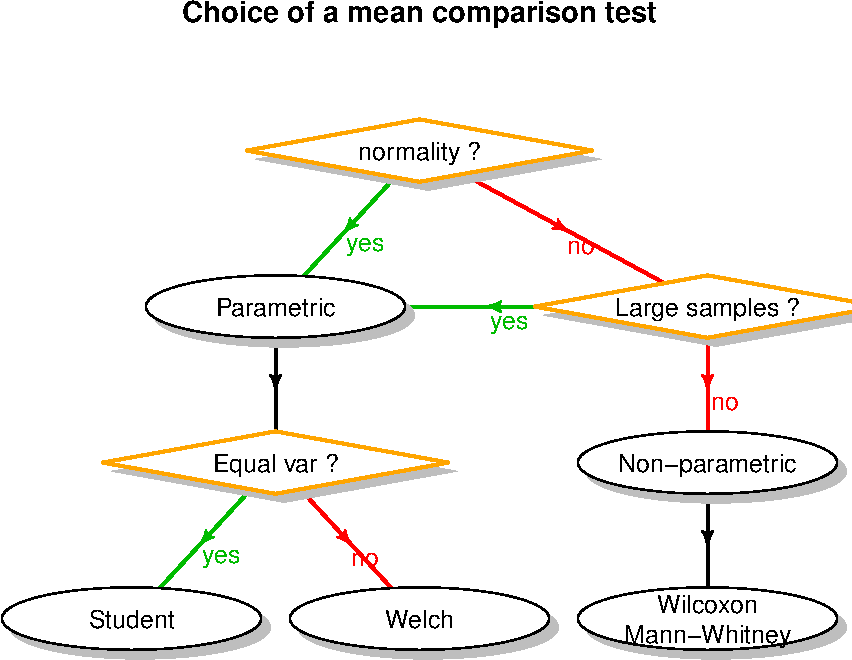
\includegraphics{figures/sampling-estimation_mean_compa_flowchart-1} \end{center}

\end{frame}

\begin{frame}{Test de Student}
\protect\hypertarget{test-de-student}{}

Hypothèses de travail: \textbf{normalité} (ou bien grands échantillons),
\textbf{homoscédasticité}.

Statistique:

\[t_{S} = \frac{\hat{\delta}}{\hat{\sigma}_\delta} =  \frac{\bar{x}_{2} - \bar{x}_{1}}{\sqrt{\frac{n_1 s_{1}^2 + n_2 s_{2}^2}{n_1+n_2-2} \left(\frac{1}{n_1}+ \frac{1}{n_2}\right)}}\]

Estimation du risque de faux-positif (\textbf{\emph{P-value}}):
probabilité d'obtenir, \textbf{\emph{sous hypothèse nulle}} une
statistique au moins aussi extrême que celle observée. Ce qu'on
appellera ``extrême'' (la ou les queues de distribution à considérer)
dépendra du sens du test.

\end{frame}

\begin{frame}{Décision}
\protect\hypertarget{duxe9cision}{}

\begin{itemize}
\tightlist
\item
  si la P-value est plus faible qu'un seuil fixé (\(\alpha\)), on
  rejette l'hypothèse nulle (\(RH_0\)) et le test est déclaré positif.
\item
  si la P-value est supérieure au seuil fixé (\(\alpha\)), on accepte
  l'hypothèse nulle (\(AH_0\)) et le test est déclaré négatif.
\end{itemize}

\begin{longtable}[]{@{}ll@{}}
\toprule
\begin{minipage}[b]{0.40\columnwidth}\raggedright
Sens du test\strut
\end{minipage} & \begin{minipage}[b]{0.54\columnwidth}\raggedright
Critère de décision\strut
\end{minipage}\tabularnewline
\midrule
\endhead
\begin{minipage}[t]{0.40\columnwidth}\raggedright
Unilatéral à droite\strut
\end{minipage} & \begin{minipage}[t]{0.54\columnwidth}\raggedright
\(RH_0 \quad \text{if} \quad t_S > t_{1-\alpha}^{n_1 + n_2 -2}\)\strut
\end{minipage}\tabularnewline
\begin{minipage}[t]{0.40\columnwidth}\raggedright
Unilatéral à gauche\strut
\end{minipage} & \begin{minipage}[t]{0.54\columnwidth}\raggedright
\(RH_0 \quad \text{if} \quad t_S < t_{alpha}^{n_1 + n_2 -2} = - t_{1-\alpha}^{n_1 + n_2 -2}\)\strut
\end{minipage}\tabularnewline
\begin{minipage}[t]{0.40\columnwidth}\raggedright
Bilatéral\strut
\end{minipage} & \begin{minipage}[t]{0.54\columnwidth}\raggedright
\(RH_0 \quad \text{if} \quad \lvert t_S \rvert > t_{1-\frac{\alpha}{2}}^{n_1 + n_2 -2}\)\strut
\end{minipage}\tabularnewline
\bottomrule
\end{longtable}

Pour le test bilatéral, on partage le risque de façon symétrique entre
les deux queues en associant \(\frac{\alpha}{2}\) à chacune.

\end{frame}

\begin{frame}{Exercice}
\protect\hypertarget{exercice}{}

Un chercheur a analysé, à l'aide de biopuces, le niveau d'expression
d'un gène d'intérêt à partir d'échantillons sanguins prélevés chez 50
patients (\(n_p=50\)) et chez 50 sujets témoins (\(n_c=50\)). Il obtient

\begin{itemize}
\tightlist
\item
  pour les patients, une moyenne \(m_p= 21\)
\item
  pour les contrôles, une moyenne \(m_c= 10\)
\item
  des écarts-types d'échantillons sont identiques pour les 2 groupes
  \(s_p = s_c = s = 15\)
\end{itemize}

Afin de tester si la différence observée entre les moyennes est
significative, le chercheur décide d'effectuer un test de Student.

\begin{enumerate}
[a.]
\item
  Le choix du test de Student vous semble-t-il approprié ? Justifiez le
  choix du chercheur. Quelles auraient été les alternatives
  envisageables ?
\item
  Sachant qu'a priori on ne sait pas dans quel sens la maladie pourrait
  affecter le niveau d'expression du gène, préconisez-vous un test uni-
  ou bilatéral ?
\item
  Formulez l'hypothèse nulle et expliquez-la en une phrase.
\item
  Sur base de la formule ci-dessous, calculez la statistique \(t\) de
  Student.
\item
  Indiquez, en vous basant sur les tables fournies, la p-valeur
  correspondante.
\item
  Interprétez la p-valeur, et aidez le chercheur à tirer les conclusions
  de son étude.
\end{enumerate}

\end{frame}

\begin{frame}{Exercice}
\protect\hypertarget{exercice-1}{}

Un groupe de chercheurs a détecté l'association entre la résistance à la
bilharziose et un taux élevé d'IgE spécifiques. D'autres chercheurs ont
cherché à répliquer ce résultat dans une population indépendante exposée
à la bilharziose. Les résultats obtenus sont indiqués ci-dessous.

\begin{itemize}
\tightlist
\item
  Pour les sujets résistants (\(n_r=32\)), la moyenne \(m_r=10\).
\item
  Pour les sujets susceptibles (\(n_s=32\)), la moyenne \(m_s=7\).
\item
  Les écarts-types des deux groupes sont égaux~:
  \(s_r = s_s = s = 2.8\).
\end{itemize}

\begin{enumerate}
[a.]
\item
  Quelle méthode préconisez-vous pour tester l'égalité des moyennes
  (justifiez)? Quelles sont les hypothèses de travail de ce test?
\item
  En partant du principe que ces conditions sont remplies dans le cas
  présent, formulez l'hypothèse nulle et calculez le score t de Student
  (formule ci-dessous). Enfin, estimez P valeur à partir de la table
  fournie.
\item
  A l'issue du test, quelle décision prenez-vous? Justifiez votre
  réponse.
\end{enumerate}

\end{frame}

\end{document}
